\section*{10. Calidad del software y pruebas}
\label{cap:calidad}

Este capítulo recoge la estrategia de validación y aseguramiento de la calidad aplicada al sistema. 
El planteamiento seguido es incremental y orientado al riesgo: primero se verifican las entidades y reglas de dominio, 
después las rutas de la API y, por último, los flujos de usuario y los escenarios de integración más relevantes.
El objetivo no es alcanzar una cobertura artificialmente máxima, sino una validación sólida, coherente con el alcance del proyecto y representativa del uso real de la plataforma.


% =============================================================
\subsection{10.1 Organización del entorno de pruebas}
\label{sec:organizacion-pruebas}

La validación se articula en una suite automatizada de 30 pruebas, distribuidas en seis bloques según el nivel de validación y la 
responsabilidad funcional del código evaluado. La batería combina pruebas unitarias, de integración, extremo a extremo, negativas, 
algorítmicas y un caso manual, con el fin de cubrir tanto la lógica de negocio como la interacción entre la API, la base de datos y los servicios auxiliares.

\begin{table}[H]
\centering
\caption{Suite de pruebas automatizadas}
\label{tab:suite-pruebas}
\renewcommand{\arraystretch}{1.3}
\begin{tabular}{lll}
\hline
\textbf{Archivo} & \textbf{Nivel de prueba} & \textbf{Nº de tests} \\
\hline
\texttt{test\_unit\_models.py}      & Unitario          & 9 \\
\texttt{test\_integration\_api.py}  & Integración       & 8 \\
\texttt{test\_e2e\_user\_journey.py}& Extremo a extremo & 2 \\
\texttt{test\_negative\_api.py}     & Negativo          & 6 \\
\texttt{test\_matching.py}          & Algorítmico       & 4 \\
\texttt{test\_manual.py}            & Datos / Manual    & 1 \\
\hline
\textbf{Total}                      &                   & \textbf{30} \\
\hline
\end{tabular}
\end{table}

A modo de resumen, las características principales de la suite son las siguientes:

\begin{itemize}
    \item \textbf{Total de pruebas:} 30.
    \item \textbf{Tiempo de ejecución:} aproximadamente 145 segundos en entorno local.
    \item \textbf{Tecnologías utilizadas:} Django \texttt{TestCase}, \texttt{APIClient}, \texttt{SimpleTestCase}, \texttt{mock} y \texttt{Coverage.py}.
    \item \textbf{Áreas cubiertas:} modelos, autenticación, relaciones sociales, API REST, algoritmo de \textit{matching} y escenarios manuales.
\end{itemize}


% =============================================================
\subsection{10.2 Niveles de pruebas y resultados}
\label{sec:niveles-pruebas}


% -------------------------------------------------------------
\subsubsection{10.2.1 Pruebas unitarias y de integración}
\label{subsec:pruebas-unitarias-integracion}

Las pruebas unitarias se centran en la validación de reglas de negocio, restricciones de integridad y funciones auxiliares del dominio. Las pruebas de integración, por su parte, ejercitan la API sobre datos reales de base de datos en un entorno de test aislado, lo que permite comprobar el comportamiento conjunto de vistas, modelos y serialización.

\begin{itemize}
    \item \textbf{Modelos (92{,}79\,\%):} Verificación de restricciones, unicidad, relaciones foráneas y validación explícita de entidades clave como \textit{Partido}, \textit{Jugador} y \textit{EquipoJugadorTemporada}.

    \item \textbf{Autenticación (84{,}68\,\%):} Registro, inicio y cierre de sesión, consulta del usuario autenticado y validación de credenciales incorrectas, incluyendo duplicidades y campos obligatorios.

    \item \textbf{Relaciones sociales:} Gestión de equipos favoritos, acceso autenticado, solicitudes de amistad y administración de notificaciones.

    \item \textbf{API de Equipos (71{,}91\,\%):} Listado, detalle, comportamiento dependiente de temporada y cálculo de datos derivados, como la sugerencia de temporada activa.

    \item \textbf{API de Jugadores (72{,}30\,\%):} Detalle individual, radar de métricas, partidos recientes y agregaciones sobre el historial del jugador.

    \item \textbf{API del Consejero (73{,}91\,\%):} Validación de entrada, control de errores y generación del veredicto de recomendación.

    \item \textbf{API de Estadísticas (82{,}78\,\%):} Comparación de jugadores y agregaciones de rendimiento sobre temporadas concretas.
\end{itemize}

La integración con PostgreSQL se verifica mediante conjuntos de datos de prueba completos, lo que permite comprobar el filtrado por temporada y jornada, las agregaciones de clasificación y la consistencia de los resultados devueltos por la API.


% -------------------------------------------------------------
\subsubsection{10.2.2 Validación de la API}
\label{subsec:validacion-api}

La validación funcional de la API cubre rutas públicas, rutas autenticadas y respuestas ante entradas inválidas. 
El objetivo no se limita a comprobar que un \textit{endpoint} responde, sino que la respuesta sea semánticamente
 correcta, estable y consumible por el \textit{frontend}.

En una ejecución focalizada de las clases \texttt{NegativeApiTests} e \texttt{IntegrationApiTests}, la batería de 14 pruebas concluyó sin errores. Durante dicha ejecución se observaron códigos de estado como \texttt{401}, \texttt{404}, \texttt{405}, \texttt{503} y \texttt{400}; sin embargo, todos ellos correspondían a escenarios negativos diseñados de forma intencional. Estos códigos no reflejan fallos del sistema, sino comportamientos esperados frente a autenticación ausente, recursos no localizados, métodos no permitidos, validaciones incorrectas o dependencias no disponibles.

\begin{table}[H]
\centering
\caption{Ejecución focalizada de validación de la API}
\label{tab:api-validation}
\renewcommand{\arraystretch}{1.3}
\begin{tabular}{lcp{7.5cm}}
\hline
\textbf{Clase} & \textbf{Tests} & \textbf{Resultado verificado} \\
\hline
\texttt{NegativeApiTests}     & 6  & Respuestas esperadas ante autenticación inválida, recursos inexistentes, métodos no permitidos y errores de validación. \\
\texttt{IntegrationApiTests}  & 8  & Flujo correcto sobre perfil, notificaciones, clasificación, jugador, consejero, estadísticas y rutas v2. \\
\hline
\textbf{Total}                & \textbf{14} & Ejecución estable, sin errores de test y con códigos de respuesta negativos intencionales. \\
\hline
\end{tabular}
\end{table}

\begin{itemize}
    \item \textbf{Pruebas positivas:} Se comprueba que los documentos JSON incluyan los campos requeridos por la interfaz y que los parámetros de temporada, jornada, posición o búsqueda alteren la respuesta de forma controlada y predecible.

    \item \textbf{Pruebas negativas:} Se validan los códigos \texttt{401}, \texttt{400}, \texttt{404}, \texttt{405} y \texttt{503} en los escenarios previstos, evitando que un error de validación o una dependencia externa no disponible se materialice en un fallo silencioso o en una excepción no controlada.
\end{itemize}


% -------------------------------------------------------------
\subsubsection{10.2.3 Pruebas de ciclo de vida}
\label{subsec:pruebas-e2e}

Se han implementado flujos extremo a extremo que reproducen el ciclo de vida más representativo del usuario en la plataforma: alta, inicio de sesión, consulta de información, gestión de favoritos y tramitación de solicitudes de amistad. Las etapas del flujo son las siguientes:

\begin{enumerate}
    \item \textbf{Registro y autenticación:} creación de usuario y obtención del token JWT.
    \item \textbf{Acceso a perfil:} lectura de \texttt{/api/me/} y comprobación del estado autenticado.
    \item \textbf{Interacción con favoritos:} alta y baja de un equipo favorito sobre datos persistidos.
    \item \textbf{Relaciones sociales:} envío, aceptación y reflejo de una solicitud de amistad sobre el estado persistido.
    \item \textbf{Cierre de sesión:} validación del \textit{logout} y desconexión del flujo autenticado.
\end{enumerate}

Este enfoque confirma que autenticación, persistencia y autorización se comportan correctamente cuando se ejecutan como un flujo completo y no como llamadas aisladas entre sí.


% -------------------------------------------------------------
\subsubsection{10.2.4 Pruebas del algoritmo de \textit{matching}}
\label{subsec:pruebas-matching}

El algoritmo de \textit{matching} se valida de forma aislada mediante casos construidos manualmente. Las pruebas comprueban la desambiguación de nombres, la priorización por minutos jugados y puntuación, y la gestión de propuestas sin coincidencia clara. Aunque su cobertura es inferior a la del resto de módulos, se trata de una lógica específica y fuertemente dependiente de datos heterogéneos, por lo que la validación por escenarios resulta más representativa que la búsqueda de una cobertura puramente cuantitativa.


% =============================================================
\subsection{10.3 Pruebas de carga}
\label{sec:pruebas-carga}

La escalabilidad del sistema se ha evaluado con Locust, simulando 20 usuarios concurrentes durante 2 minutos sobre los \textit{endpoints} de consulta más frecuentes. El objetivo es medir el comportamiento del \textit{backend} bajo carga realista, sin introducir variabilidad artificial.

\begin{table}[H]
\centering
\caption{Resultados de las pruebas de carga}
\label{tab:carga}
\renewcommand{\arraystretch}{1.3}
\begin{tabular}{ll}
\hline
\textbf{Métrica} & \textbf{Valor} \\
\hline
Usuarios concurrentes & 20 \\
Total de peticiones   & 1\,220 \\
Throughput            & 10{,}22 req/s \\
Latencia promedio     & 708 ms \\
\hline
\end{tabular}
\end{table}

Los resultados son coherentes con un entorno de desarrollo local y confirman que la capa de lectura responde de forma estable bajo la carga simulada. La caché con Redis amortigua parte del coste en \textit{endpoints} repetitivos; no obstante, en un escenario productivo será necesario escalar la infraestructura y revisar las estrategias de invalidación y particionado de carga.


% =============================================================
\subsection{10.4 Resultados de cobertura y calidad}
\label{sec:cobertura-calidad}

Para auditar la calidad del código se han combinado dos métricas complementarias: cobertura dinámica con \texttt{Coverage.py} y análisis estático con SonarQube. La primera cuantifica el comportamiento ejecutado por la suite de pruebas; la segunda permite identificar deuda técnica, \textit{hotspots} de seguridad y problemas de mantenibilidad sin necesidad de ejecutar el sistema.


% -------------------------------------------------------------
\subsubsection{10.4.1 Cobertura de código}
\label{subsec:cobertura}

Se estableció un umbral mínimo del 70\,\%. Tras la ejecución de la suite consolidada de 30 pruebas, el sistema alcanzó un 83{,}02\,\% de cobertura global sobre el alcance definido en \texttt{.coveragerc}, superando el objetivo planteado sin aproximarse a un valor artificialmente perfecto.

\begin{table}[H]
\centering
\caption{Cobertura de código por módulo}
\label{tab:cobertura}
\renewcommand{\arraystretch}{1.3}
\begin{tabular}{lcp{5.5cm}}
\hline
\textbf{Módulo} & \textbf{Cobertura} & \textbf{Descripción} \\
\hline
\texttt{main.models}              & 92{,}79\,\% & Restricciones, relaciones FK e integridad referencial. \\
\texttt{main.api.auth}            & 84{,}68\,\% & Registro, \textit{login}, \textit{logout} y estado de sesión. \\
\texttt{main.api.consejero}       & 73{,}91\,\% & Validación de entrada y veredicto de recomendación. \\
\texttt{main.api.equipo}          & 71{,}91\,\% & Listado y detalle de equipos. \\
\texttt{main.api.jugador}         & 72{,}30\,\% & Detalle individual, radar, histórico y partidos. \\
\texttt{main.api.menu}            & 79{,}81\,\% & Resumen principal y \textit{top} jugadores. \\
\texttt{main.api.estadisticas}    & 82{,}78\,\% & Comparación de jugadores y agregaciones de rendimiento. \\
\texttt{main.drf\_views}          & 100{,}00\,\% & Adaptadores v2 y rutas equivalentes. \\
\texttt{main.scrapping.matching}  & 66{,}02\,\% & Agrupación y resolución del algoritmo de \textit{matching}. \\
\hline
\textbf{Total del sistema}        & \textbf{83{,}02\,\%} & Cobertura global integrada mediante 30 pruebas. \\
\hline
\end{tabular}
\end{table}

El módulo de \textit{matching} queda por debajo del resto porque concentra una lógica algorítmica compleja cuya cobertura por exhaustividad resulta poco práctica. Aun así, su validación específica con casos sintéticos evita regresiones en los criterios de resolución y mantiene controlado el comportamiento en los escenarios más sensibles.


% -------------------------------------------------------------
\subsubsection{10.4.2 Análisis estático con SonarQube}
\label{subsec:sonarqube}

El análisis estático realizado con SonarQube ofrece una visión complementaria del estado del proyecto. Los resultados permiten mantener el nivel de calidad dentro de un rango alto pero realista, sin forzar una cobertura total que no aportaría valor adicional al proceso de validación.

\begin{itemize}
    \item \textbf{Mantenibilidad (Rating A):} La base de código presenta un buen nivel de calidad estructural, con una deuda técnica reducida en relación con el volumen analizado. Se han identificado 147 \textit{code smells}, con un esfuerzo de mejora estimado en 4 días de trabajo.

    \item \textbf{Seguridad (Rating E):} Se han identificado 10 \textit{security hotspots}, revisados manualmente, asociados principalmente a la gestión de sesiones y a la configuración de red. Entre ellos se incluyen credenciales embebidas en el código fuente de los tests, que SonarQube no distingue automáticamente de credenciales reales de producción.

    \item \textbf{Fiabilidad (Rating A):} La herramienta no detecta ningún \textit{bug} en el código analizado.
\end{itemize}

En conjunto, la combinación de cobertura automatizada, validación de casos negativos y análisis estático proporciona una base sólida para evolucionar la plataforma con menor riesgo de regresión, manteniendo un equilibrio razonable entre la amplitud de las pruebas y el coste de su mantenimiento.

\begin{figure}[H]
    \centering
    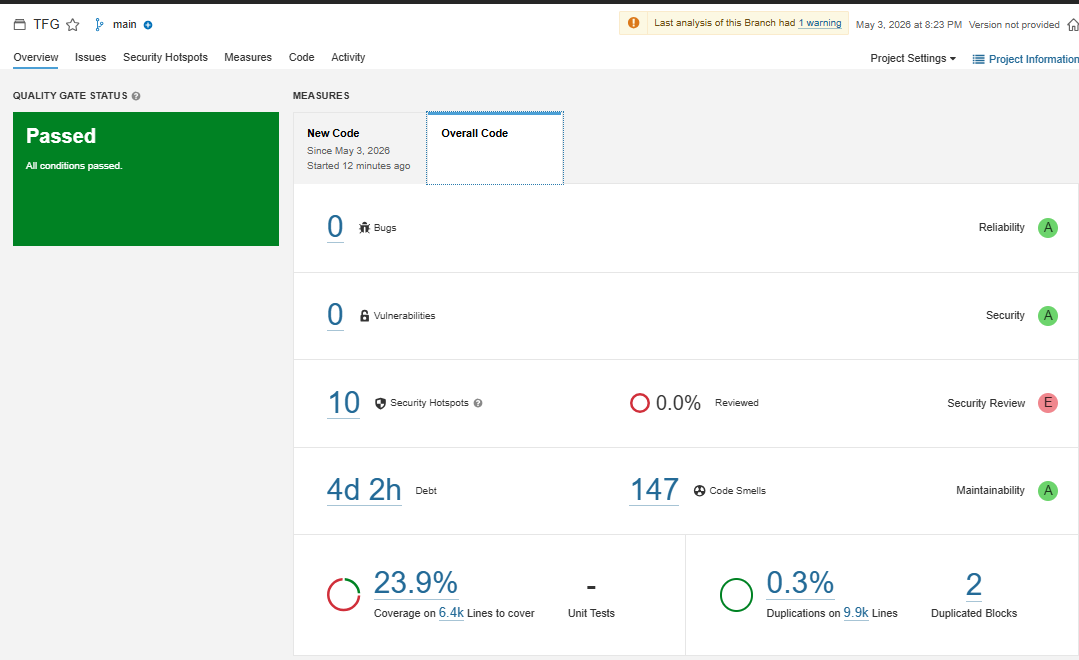
\includegraphics[width=0.9\textwidth]{images/sonar.png}
    \caption{Estado del \textit{dashboard} de SonarQube tras el análisis del proyecto.}
    \label{fig:sonar-dashboard}
\end{figure}